\listfiles

\documentclass[a4paper,ngerman,12pt,bibtotoc]{scrartcl}

\usepackage[utf8]{inputenc}

\usepackage[ngerman]{babel}
\addto\captionsngerman{\renewcommand\tablename{Tafel}}

\usepackage{amsmath, amsthm, amssymb, stmaryrd, color, graphicx, mathtools}
\usepackage{setspace}
\usepackage{bussproofs}
\usepackage{array}
\usepackage{booktabs}
\usepackage{comment}
\usepackage{textcomp}
\usepackage{stmaryrd}

\usepackage[protrusion=true,expansion=true]{microtype}

\usepackage{lmodern}
\usepackage{tabto}

\usepackage[backend=bibtex,style=alphabetic]{biblatex}
\usepackage[babel]{csquotes}
\bibliography{literatur}

\usepackage{titling}

\usepackage[all]{xy}

\usepackage[colorlinks=true, linkcolor=blue, urlcolor=blue, citecolor=blue]{hyperref}
\usepackage{cleveref}			%Referenzen mit Name


\usepackage{algorithm}
\usepackage{algpseudocode}
\algrenewcommand{\algorithmiccomment}[1]{\hskip3em$\slash\slash$ #1}
\newcommand{\LineFor}[2]{\State\algorithmicfor\ {#1}\ \algorithmicdo\ {#2}}


\usepackage[left=2.5cm, right=2.5cm, bottom=2cm, top=2.5cm]{geometry}


\setlength\parskip{\medskipamount}
\setlength\parindent{0pt}

\theoremstyle{definition}
\newtheorem{defn}{Definition}
\newtheorem{axiom}[defn]{Axiom}
\newtheorem{bsp}[defn]{Beispiel}

\theoremstyle{plain}

\newtheorem{prop}[defn]{Proposition}
\newtheorem{motto}[defn]{Motto}
\newtheorem{ueberlegung}[defn]{Überlegung}
\newtheorem{lemma}[defn]{Lemma}
\newtheorem{kor}[defn]{Korollar}
\newtheorem{hilfsaussage}[defn]{Hilfsaussage}
\newtheorem{satz}[defn]{Satz}

\theoremstyle{remark}
\newtheorem{erin}[defn]{Erinnerung}
\newtheorem{bem}[defn]{Bemerkung}
\newtheorem{beob}[defn]{Beobachtung}
\newtheorem{aufg}[defn]{Aufgabe}

\clubpenalty=10000
\widowpenalty=10000
\displaywidowpenalty=10000

\newcommand{\ZZ}{\mathbb{Z}}
\newcommand{\QQ}{\mathbb{Q}}
\newcommand{\RR}{\mathbb{R}}
\newcommand{\CC}{\mathbb{C}}
\newcommand{\NN}{\mathbb{N}}
\newcommand{\PP}{\mathbb{P}}
\newcommand{\Ic}{\mathcal{I}}
\newcommand{\Jc}{\mathcal{J}}
\newcommand{\Hc}{\mathcal{H}}
\newcommand{\Tc}{\mathcal{T}}
\newcommand{\Sc}{\mathcal{S}}
\newcommand{\Oc}{\mathcal{O}}


\newcommand{\Hom}{\mathrm{Hom}}
\newcommand{\id}{\mathrm{id}}
\newcommand{\Id}{\mathrm{Id}}

\newcommand{\OPT}{\mathrm{OPT}}
\newcommand{\MST}{\mathrm{MST}}

\newcommand{\TSP}{\textbf{TSP}}
\newcommand{\HomTSP}{\textbf{HomTSP}}
\newcommand{\HetTSP}{\textbf{HetTSP}}
\newcommand{\CVRP}{\textbf{CVRP}}
\newcommand{\HetCVRP}{\textbf{HetCVRP}}


\renewcommand*\theenumi{\alph{enumi}}
\renewcommand{\labelenumi}{(\theenumi)}

\setcounter{tocdepth}{2}

\newenvironment{indentblock}{%
	\list{}{\leftmargin\leftmargin}%
	\item\relax
}{%
\endlist
}



\begin{document}
	\pagenumbering{gobble}
	
	\begin{minipage}{0.7\textwidth}
		\begin{flushleft}
			Universität Augsburg \\
			Seminar: Approximationsalgorithmen und Spieltheorie \\
			Dozent: Prof. Dr. Tobias \textsc{Harks} 
		\end{flushleft}
	\end{minipage}
	\begin{minipage}{0.3\textwidth}
		\begin{flushright}
			Lukas \textsc{Graf} \\
			12. Mai 2016 \\
			Sommersemester 2016
		\end{flushright}
	\end{minipage}
	
	\hrulefill
	\vspace{-1em}
	\begin{center}\LARGE\textbf{Heterogenes $k$-CVRP}\end{center}
	\vspace{-1.4em}
	\hrulefill
	\vspace{-1.4em}
	
	\hrulefill
	
	\vspace{1em}	
	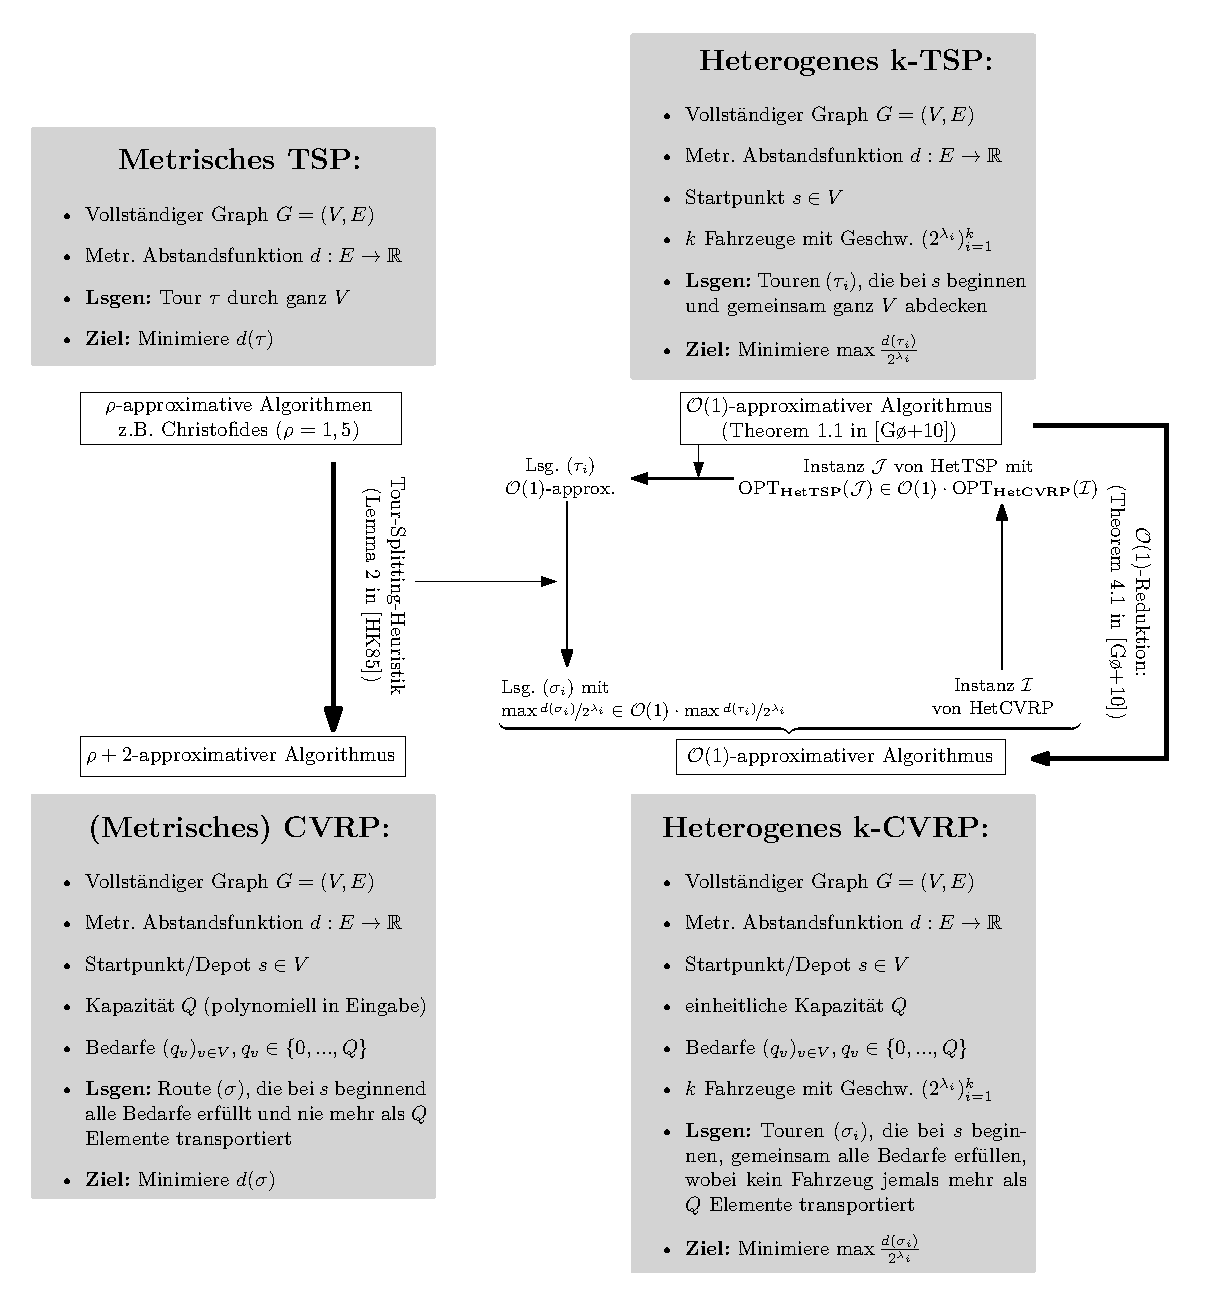
\includegraphics[width=1\textwidth]{Problemdefinitionen2.pdf}

	\hrulefill
			
	{
		\renewcommand{\section}[2]{}
		\renewcommand*{\bibfont}{\tiny}
		\nocite{*}
		\printbibliography		
	}		
		
	\section*{Algorithmus für heterogenes $k$-TSP}\footnotesize
	
	\begin{minipage}{0.5\textwidth}
		\begin{algorithm}[H]\footnotesize
			\caption{\small \textsc{HetTSP-Approx}$(G, d)$}\label{AlgHetTSP}
			\begin{algorithmic}[1]
				\State Rate $M$ mit $\OPT \leq M \leq 2\cdot\OPT$
				\State $\Hc := \left(H_l\right)_{l\geq 0} \gets$ \textsc{Level-Prime} $\left(G, d\right)$
				\State $\Tc := \left(\Tc_l\right)_{l\geq 0} \gets$ \textsc{Decomposition} $\left(\Hc\right)$
				\State $\left(x_{Ti}\right) \gets$ \textsc{FractionalAssignment}  $\left(\Tc\right)$
				\State $\left(\tau_i\right) \gets$ \textsc{RoundingAssignment} $\left(x_{Ti}\right)$
				\State \Return $\left(\tau_i\right)$
			\end{algorithmic}
		\end{algorithm}
		
		\begin{algorithm}[H]\footnotesize
			\caption{\small\textsc{Level-Prim}$(G, d)$}\label{AlgLevelPrim}
			\begin{algorithmic}[1]
				\State $V_0 := \left\lbrace v\in V \mid d(s,v) \leq M\right\rbrace$
				\State $V_l := \left\lbrace v \in V \mid 2^{l-1}M < d(s,v) \leq 2^l M\right\rbrace$
				\LineFor{$i\geq 0$}{$H_l \gets$ MST auf $G\left[V_{\leq l}\right]/V_{<l}$}
				\State \Return $\left(H_l\right)_{l\geq 0}$
			\end{algorithmic}
		\end{algorithm}	
		
		\begin{algorithm}[H]\footnotesize
			\caption{\small \textsc{Decomposition}$\left(\Hc\right)$}\label{AlgDecomposition}
			\begin{algorithmic}[1]
				\State $\Sc_0 := \left\lbrace H_0 \right\rbrace$
				\State $\Sc_l := \text{Zerl. } \Hc\cap E_l \text{ in Bäume mit Wurzel in } V_{<l}$
				\State $\Sc_l^{\geq} := \left\{\tau \in \Sc_l \mid d(\tau) \geq 2^{l-3}M\right\}, \Sc_l^< := \Sc_l \backslash \Sc_l^{\geq}$
				\LineFor{$\tau \in \Sc_l^{<}$}{$h(\tau) := \tau' \in S_{l-1}^{\geq}$ mit $\tau \cup \tau'$ zsh}
				\For{$\tau \in \Sc_l^{\geq}$}
				\State $\Tc_l(\tau) \gets$ Partition von $\tau \cup h^{-1}(\tau)$ in Bäume der Länge $\left[2^{l+1}M, 2^{l+2}M\right]$ (und evtl. ein kürzerer)
				\State $\Tc'_l(\tau) \gets \left\{T_r \cup \{\text{ Kante zu } s\} \mid T_r \in \Tc_l(\tau)\right\}$
				\EndFor
				\State $\Tc_l := \bigcup_{\tau \in \Sc_l^{\geq}}\Tc'_l(\tau)$
				\State \Return $\left(\Tc_l\right)_{l\geq 0}$
			\end{algorithmic}
		\end{algorithm}
		
		\begin{algorithm}[H]\footnotesize
			\caption{\small \textsc{FractionalAssignment}$\left(\Tc\right)$}\label{AlgFractionalAssignment}
			\begin{algorithmic}[1]
				\State $L := \{T \in \Tc\},\quad b(T) := d(T)$
				\State $R := \{i \mid 1\leq i \leq k\},\quad b(i) := \beta M 2^{\lambda_i}$
				\State $F := \{\{T,i\} \mid T \in \Tc_l, \lambda_i \geq l-1\}$ 
				\State $\left(x_{Ti}\right) \gets$ $L$-überdeckendes $b$-Matching
				\State \Return $\left(x_{Ti}\right)$
			\end{algorithmic}
		\end{algorithm}
		
		\begin{algorithm}[H]\footnotesize
			\caption{\small \textsc{RoundingAssignment}$\left(x_{Ti}\right)$}\label{AlgRoundingAssignment}
			\begin{algorithmic}[1]
				\State $\left(x'_{Ti}\right) \gets$ \textsc{RoundScheduling}($p_{Ti} := \frac{d(T)}{2^{\lambda_i}}, \tilde{x}_{Ti} := \frac{x_{Ti}}{d(T)}$)
				\State $\tau_i \gets$ Tour durch die Bäume $T$ mit $x'_{Ti} = 1$.
				\State \Return $\left(\tau_i\right)$
			\end{algorithmic}
		\end{algorithm}								
	\end{minipage}
	\begin{minipage}{0.05\textwidth}
		\phantom{Hallo}
	\end{minipage}
	\begin{minipage}{0.45\textwidth}
		\vspace{4em}
		
		\begin{satz}[Theorem 1.1 in \cite{HetCVRP}]~
			
			\Cref{AlgHetTSP} ist ein $\Oc(1)$-approximativer Algorithmus für \HetTSP.
		\end{satz}
		
		\vspace{3em}

		\begin{lemma}[Korollar 3.5 in \cite{HetCVRP}]~
			
			Ein von \cref{AlgLevelPrim} gefundener Baum $\left(H_l\right)_{l\geq 0}$ erfüllt:
			\begin{itemize}
				\item Die Knoten-Level entlang jedes Wurzel-Blatt-Pfades sind monoton wachsend.
				\item $\forall l\geq -1: \sum_{j>l} d(H_j) \leq 8M\cdot \sum_{j\geq l}2^j\mu_j$
			\end{itemize}
		\end{lemma}

		\begin{defn}[Definition 3.1 in \cite{HetCVRP}]~
			
			Ein Wald $\Tc = \bigcup_{l\geq 0} \Tc_l$ aus Bäumen mit Wurzel $s$ heißt $(\alpha, \beta)$-zuweisbar, wenn gilt:
			\begin{itemize}
				\item Für alle $T \in \Tc_l$ gilt: $d(T) \leq \alpha 2^l M$ \\
				\textit{d.h. ein Baum aus $\Tc_l$ kann mit Geschw. $2^l$ in $\Oc(\alpha M)$ besucht werden.}
				\item Für alle $l \geq -1$ gilt: $\sum_{j > l} d(\Tc_j) \leq \beta M \sum_{j\geq l} 2^j\mu_j$
				
				\textit{d.h. die Fahrzeuge mit Geschw. $\geq 2^l$ können den Wald $\Tc_{>l}$ in $\Oc(\beta M)$ besuchen.}
			\end{itemize}
		\end{defn}
		
		\begin{lemma}[Lemma 3.11 in \cite{HetCVRP}]~
			
			Die von \cref{AlgDecomposition} bestimmte Zerlegung $\Tc = (\Tc_i)_{i\geq 0}$ ist $(6, 40)$-zuweisbar.
		\end{lemma}

		\begin{defn}
			$(x_{Ti})$ ist \emph{$L$-sättigendes $b$-Matching} für $(L\cup R, F)$, wenn gilt:
			\[\sum_i x_{Ti} = b(T),\quad \sum_T x_{Ti} \leq b(i),\quad x_{Ti}\in\NN\]
		\end{defn}
		
		\begin{lemma}[Seite 54f in \cite{bMatching}]~
			
			Der in \cref{AlgFractionalAssignment} definierte Hilfsgraph besitzt ein $L$-sättigendes $b$-Matching.
		\end{lemma}

		\begin{lemma}[Theorem 1 in \cite{Rounding}, Lemma 3.2 in \cite{HetCVRP}]~
			
			Gegeben einen $(\alpha, \beta)$-zuweisbaren Wald, liefern \cref{AlgFractionalAssignment} und \cref{AlgRoundingAssignment} eine $(4\alpha+2\beta)$-approximative Lösung für \HetTSP.
		\end{lemma}
	\end{minipage}
	
\end{document}